\section{Dataset 15\%}
Describe the data you are working with for your project. What type of data is it? Where did it come from? How much data are you working with? Did you have to do any preprocessing, filtering, etc., and why?
%------------------------------------------------------------------------

In this section we present the datasets we have used: one for the detection task and one for the classifier models. 



The Belgium Traffic Sign Dataset refers to a set of 62 classes of traffic signs: training data files are divided into 62 folders that contain the images in PPM format. The same for validation data. We decided to cut some classes and to add some new ones in order to build an accurate classifier which focuses on most meaningful traffic signs. The dataset we have used to train and to validate the classifier model is made of 56 traffic sign classes with 6229 images for training and 2493 for the validation. Every image is a cropped portion taken from a road picture which represents one traffic sign. Typically the images are characterized by small square dimensions and sizes. The aim of the classifier is to pick the right class for each input image, but in Europe there could be small appearance differences between the same traffic sign classes from a state and another. 
\begin{figure}{}
	\centering
	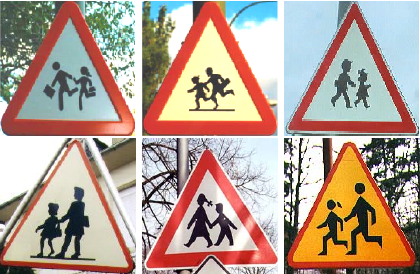
\includegraphics[width=0.6\linewidth]{Img/differences.png}
	\caption{Differences between signs of the same class}\label{}
\end{figure}

To fix this issue, we manually added some images to training and validation data for classes which suffer this problem. Also, we adopted the augmentation techniques to build a wider dataset. Doing this we noticed an increased accuracy of the classifier. 